\section{Aproximação de longa distância}
\label{sec:cap4_app_longa}

Nesta fase da missão de \gls{rvdb}, as variáveis são analisadas no referencial inercial, desde o instante de injeção do perseguidor na órbita inicial até o término da transferência orbital por \gls{th}, quando se obtém o conjunto final de elementos orbitais.
A Tabela~\ref{tab:cap4_1_raio_orbital} apresenta os raios orbitais circularizados do perseguidor no instante inicial e após a \gls{th}, em comparação com o raio orbital do alvo. As altitudes iniciais são $500$ km (perseguidor) e $600$ km (alvo).

\begin{table}[H]
\centering
\caption{Raio orbital}
\begin{tabularx}{\linewidth}{|>{\raggedright\arraybackslash}X|>{\centering\arraybackslash}X|}
\hline
\multicolumn{1}{|c|}{\textbf{Raio orbital}} &
\multicolumn{1}{c|}{\textbf{quilômetro}} \\
\hhline{|=|=|}
Perseguidor (inicial) & 6.878,13 \\
\hline
Perseguidor (após \gls{th}) & 6.978,03 \\
\hline
Alvo & 6.978,13 \\
\hline
\end{tabularx}
\label{tab:cap4_1_raio_orbital}
\end{table}

A condição de fase inicial entre as espaçonaves, apresentada na Tabela~\ref{tab:cap4_2_longitude}, foi definida como parte das condições iniciais da simulação e representa a separação angular do perseguidor em relação ao alvo, tomado como referência. Adotou-se um deslocamento inicial de $-7^\circ$ para o perseguidor, isto é, uma separação angular inicial "atrás" do alvo no sentido do movimento orbital, assumindo-se que tal condição é estabelecida pelo veículo lançador após a separação do perseguidor em sua órbita de injeção.


\begin{table}[H]
\centering
\caption{Longitude inicial de cada espaçonave no instante 0 da simulação.}
\begin{tabularx}{\linewidth}{|>{\raggedright\arraybackslash}X|>{\centering\arraybackslash}X|}
\hline
\multicolumn{1}{|c|}{\textbf{Fase/longitude}} &
\multicolumn{1}{c|}{\textbf{[grau] (radiano)}} \\
\hhline{|=|=|}
Perseguidor & [$-7,00$] ($-1,222$) \\
\hline
Alvo & [$0,00$] ($0,00$) \\
\hline
\end{tabularx}
\label{tab:cap4_2_longitude}
\end{table}

A Figura~\ref{fig:cap4_1Posições_perseguidor_alvo1} mostra as posições iniciais do perseguidor e do alvo, bem como os instantes de aplicação de $\Delta v_1$ e $\Delta v_2$. A aplicação de $\Delta v_2$ marca o encerramento desta fase da missão de \gls{rvdb}.

\begin{figure}[H]
\centering
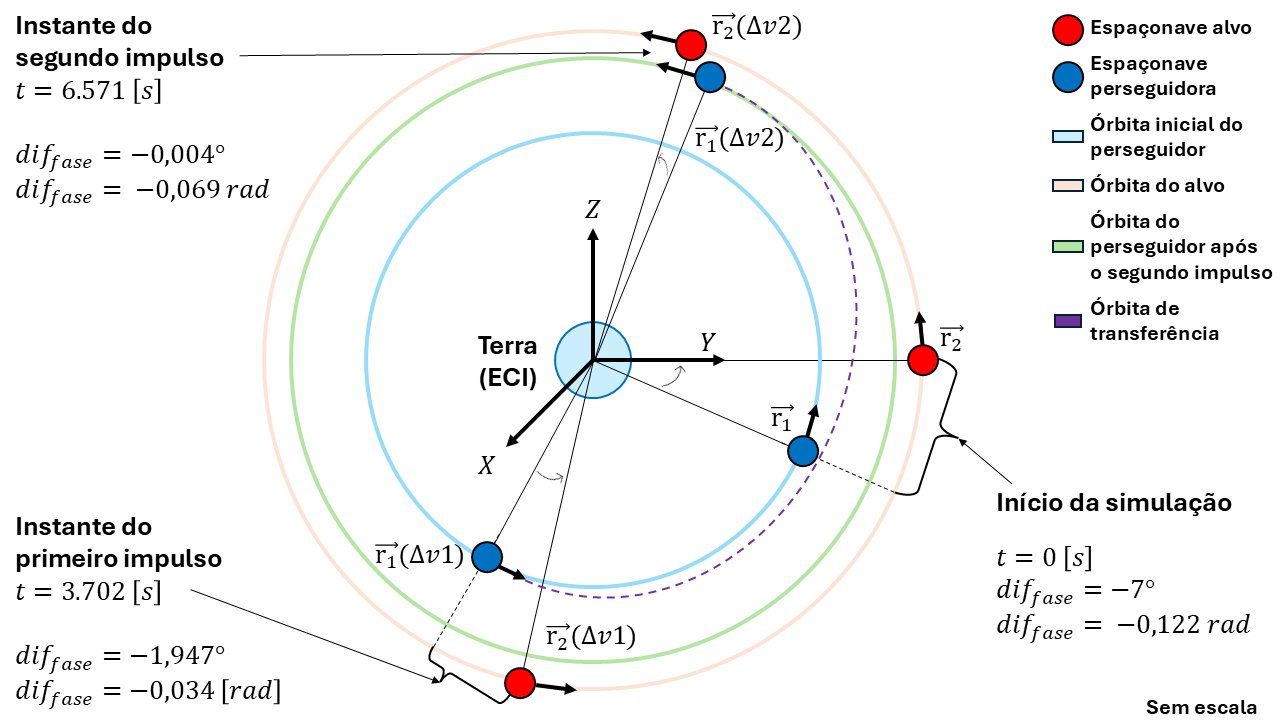
\includegraphics[width=1\linewidth]{4 Resultados e discussoes/Imagens/1 App longa distancia/1 Transferência de órbita.png}
\caption{Posições inicial e final das espaçonaves durante a fase de aproximação longa da missão de \gls{rvdb}.}
    \label{fig:cap4_1Posições_perseguidor_alvo1}
\end{figure}

A seguir, a Figura~\ref{fig:cap4_1Posições_perseguidor_alvo2} exibe o momento em que é iniciado a deriva orbital e seu término para iniciar a aproximação de curta distância.

\begin{figure}[H]
\centering
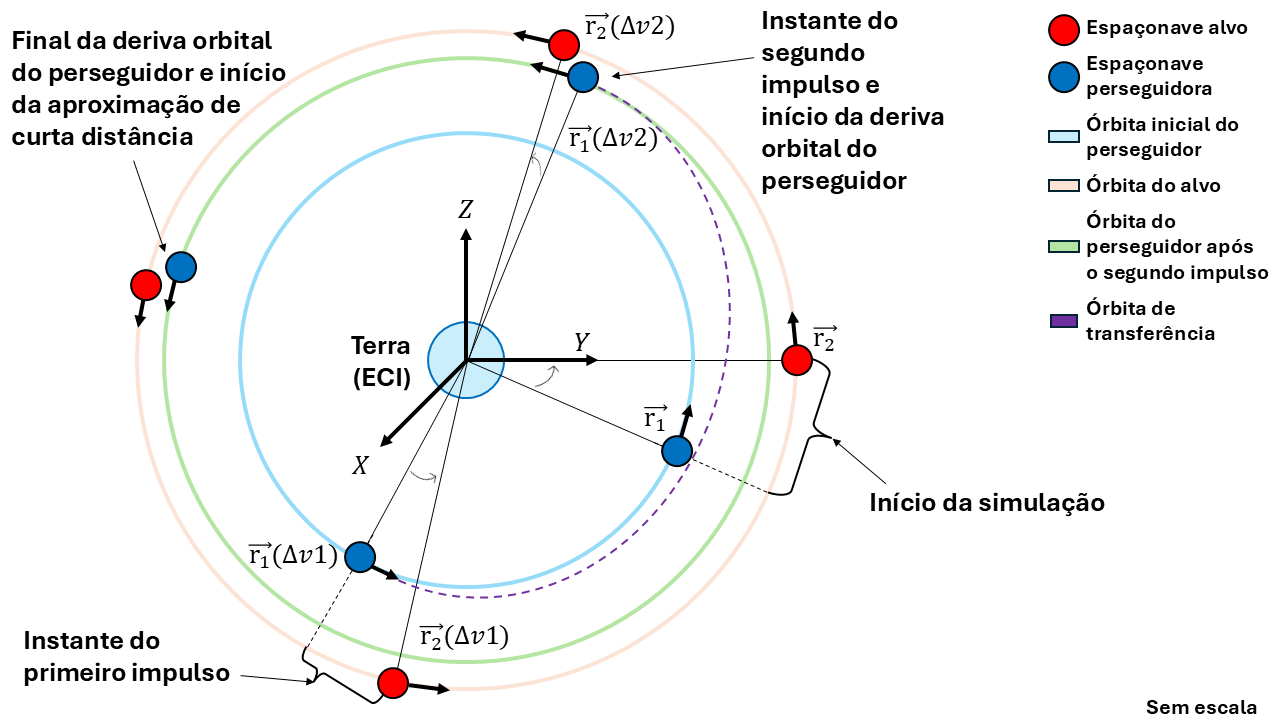
\includegraphics[width=1\linewidth]{4 Resultados e discussoes/Imagens/1 App longa distancia/1 Final da transf orbita.png}
\caption{Deriva orbital do perseguidor após o segundo impulso durante a aproximação de longa distância da missão de \gls{rvdb}.}
    \label{fig:cap4_1Posições_perseguidor_alvo2}
\end{figure}

A seguir, a Figura~\ref{fig:cap4_2Longitudes_perseguidor_alvo} apresenta a diferença de longitude entre as espaçonaves ao longo do tempo, juntamente com os instantes da queima 1 e 2.
O tempo inicial deste gráfico é o início absoluto da simulação da missão de \gls{rvdb}

\begin{figure}[H]
\centering
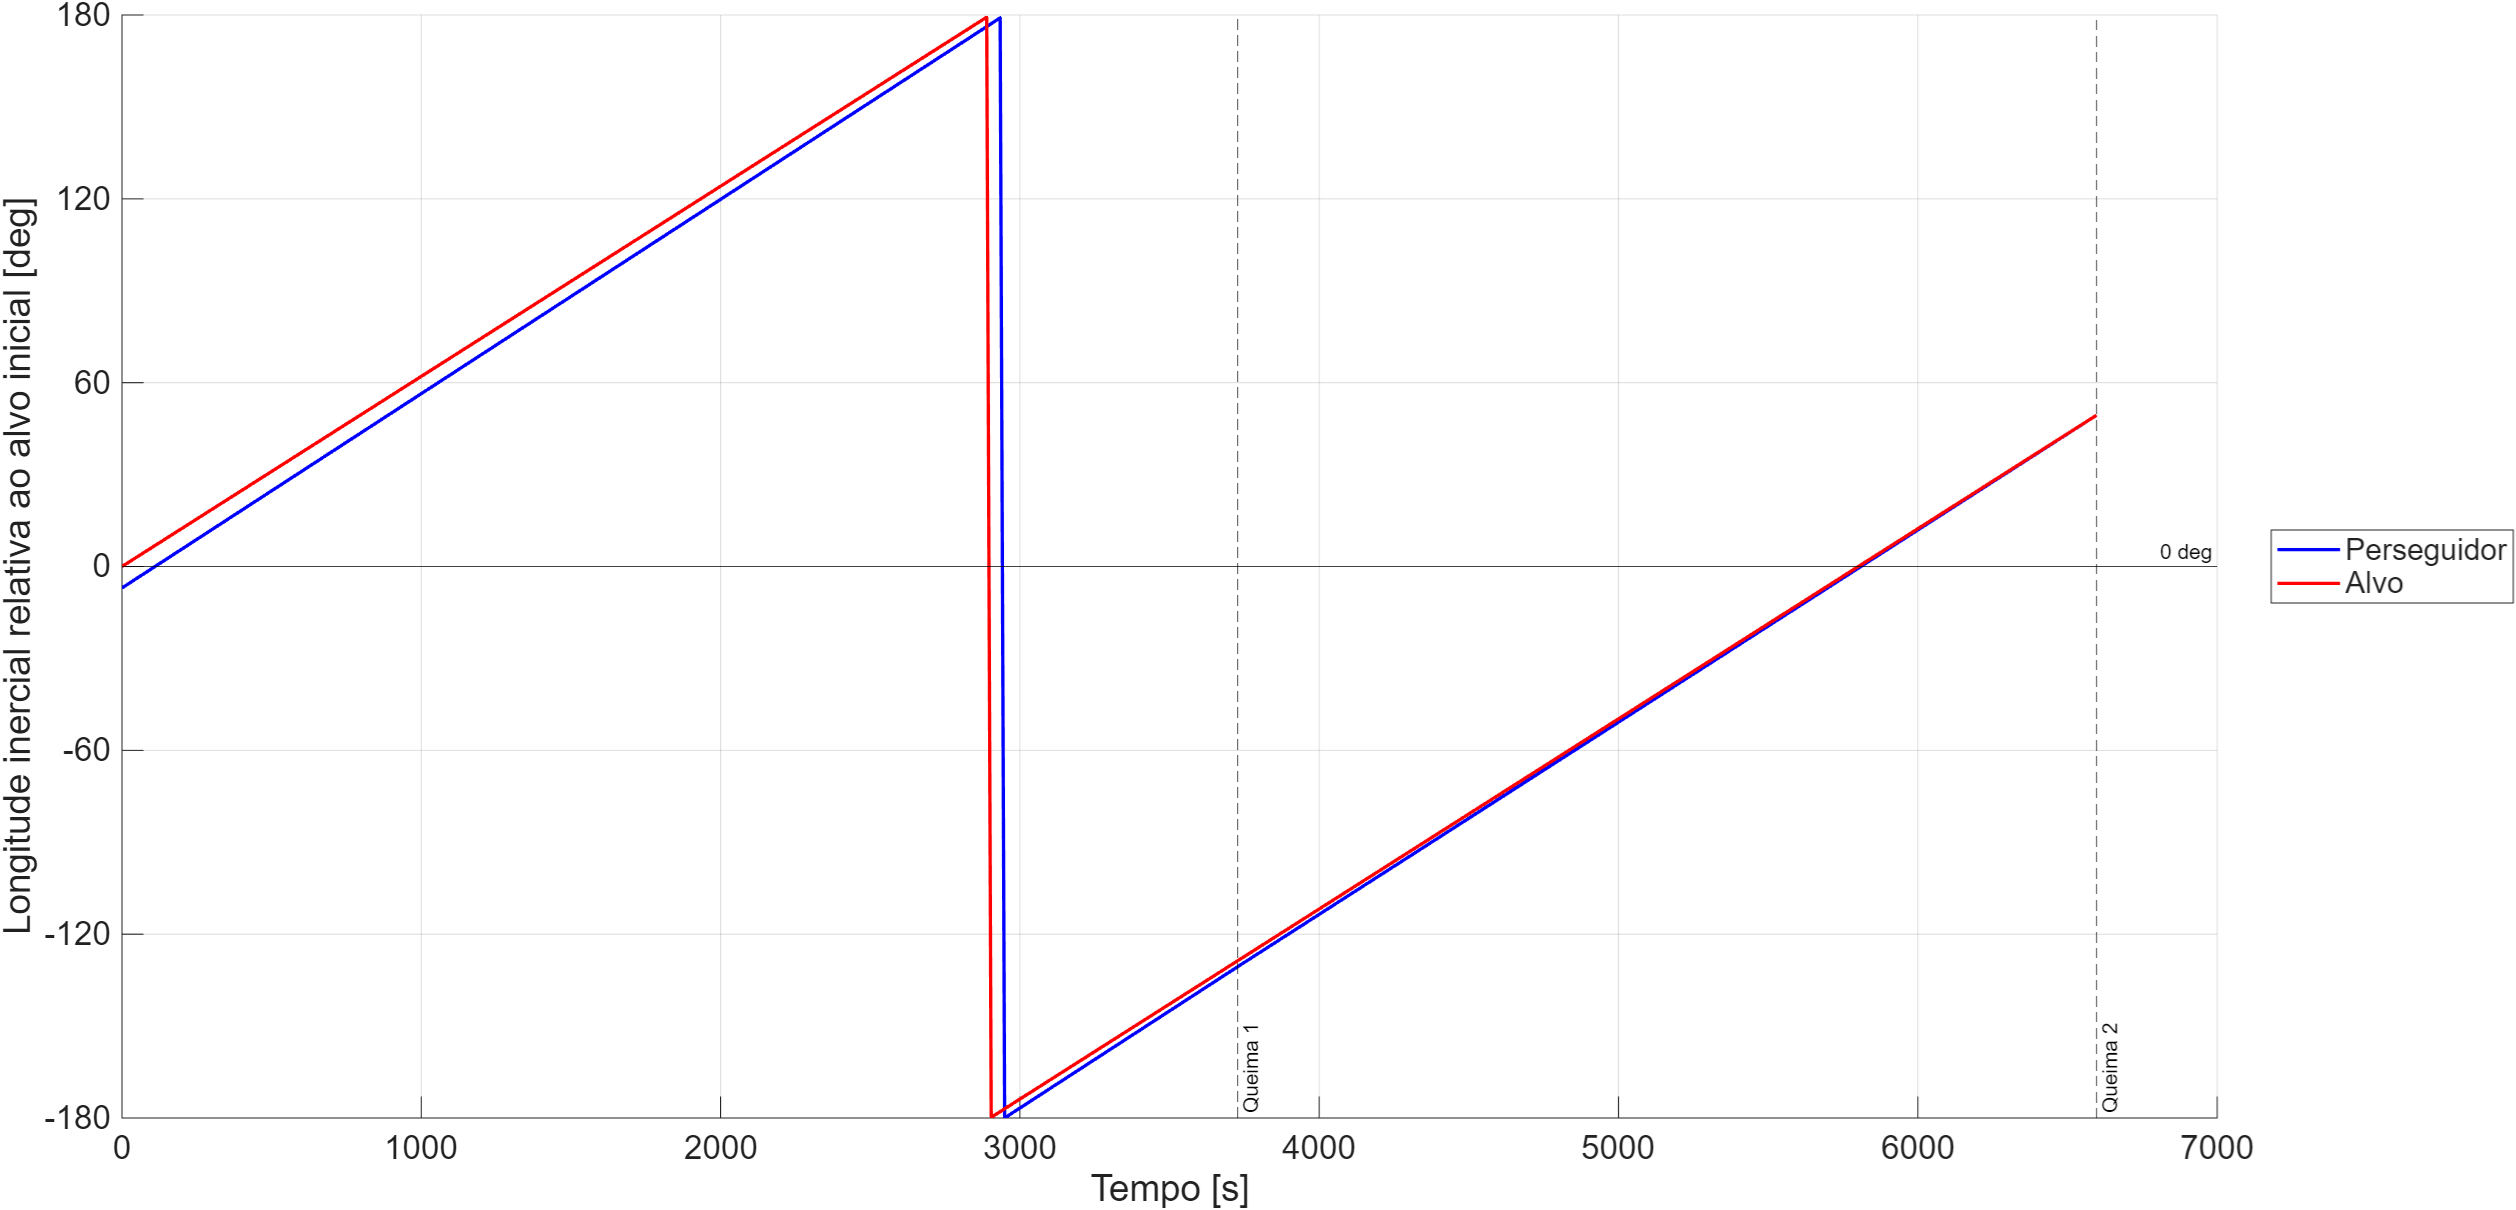
\includegraphics[width=1\linewidth]{4 Resultados e discussoes/Imagens/1 App longa distancia/2 Longitude ao longo do tempo.png}
\caption{Evolução da longitude relativa ao longo do tempo.}
    \label{fig:cap4_2Longitudes_perseguidor_alvo}
\end{figure}


Ao final da aproximação de longa distância, no instante $6.596$ s, a longitude do alvo é $49,38^{\circ}$ e a do perseguidor é $49,38^{\circ}$, resultando em diferença de $0,004^{\circ}$ ($0,069$ rad), correspondente a $506,06$ m de separação relativa.

A Tabela~\ref{tab:cap4_3_longitude_instantes} apresenta as longitudes em instantes selecionados e a respectiva diferença de fase.
Em termos de tempo absoluto, o perseguidor levou $6.571$~s ($01$h$49$min$31$s) para atingir a condição de término desta fase, ou seja, aproximou-se suficientemente do alvo, finalizando a primeira fase da missão de \gls{rvdb}.


\begin{table}[H]
\centering
\caption{Diferença de fase ao longo do tempo (ECI)}
\begin{tabularx}{\linewidth}{|>{\centering\arraybackslash}X|>{\centering\arraybackslash}X|>{\centering\arraybackslash}X|>{\centering\arraybackslash}X|}
\hline
\multicolumn{1}{|c|}{\textbf{Instante}} &
\multicolumn{3}{c|}{\textbf{Longitude [grau]}} \\
\textbf{[s]} & \textbf{Perseguidor} & \textbf{Alvo} & \textbf{Diferença} \\
\hhline{|=|=|=|=|}
$0$      & $-7,0000^{\circ}$   & $0,0000^{\circ}$    & $-7,0000^{\circ}$ \\
$2.889$  & $176,2150^{\circ}$  & $179,2910^{\circ}$  & $-3,0760^{\circ}$ \\
$3.728$  & $308,6870^{\circ}$  & $310,6240^{\circ}$  & $-1,9370^{\circ}$ \\
$6.571$  & $49,3760^{\circ}$   & $49,3801^{\circ}$   & $-0,0041^{\circ}$ \\
\hline
\end{tabularx}
\label{tab:cap4_3_longitude_instantes}
\end{table}

\subsection{Raio orbital do perseguidor ao longo do tempo}

A evolução do raio orbital do perseguidor é observada na Figura~\ref{fig:cap4_3_raio_orbital}.
No instante inicial da simulação, o perseguidor está na altitude de $500$ km, ou seja, raio orbital de  $6.878,13$ km.

\begin{figure}[H]
\centering
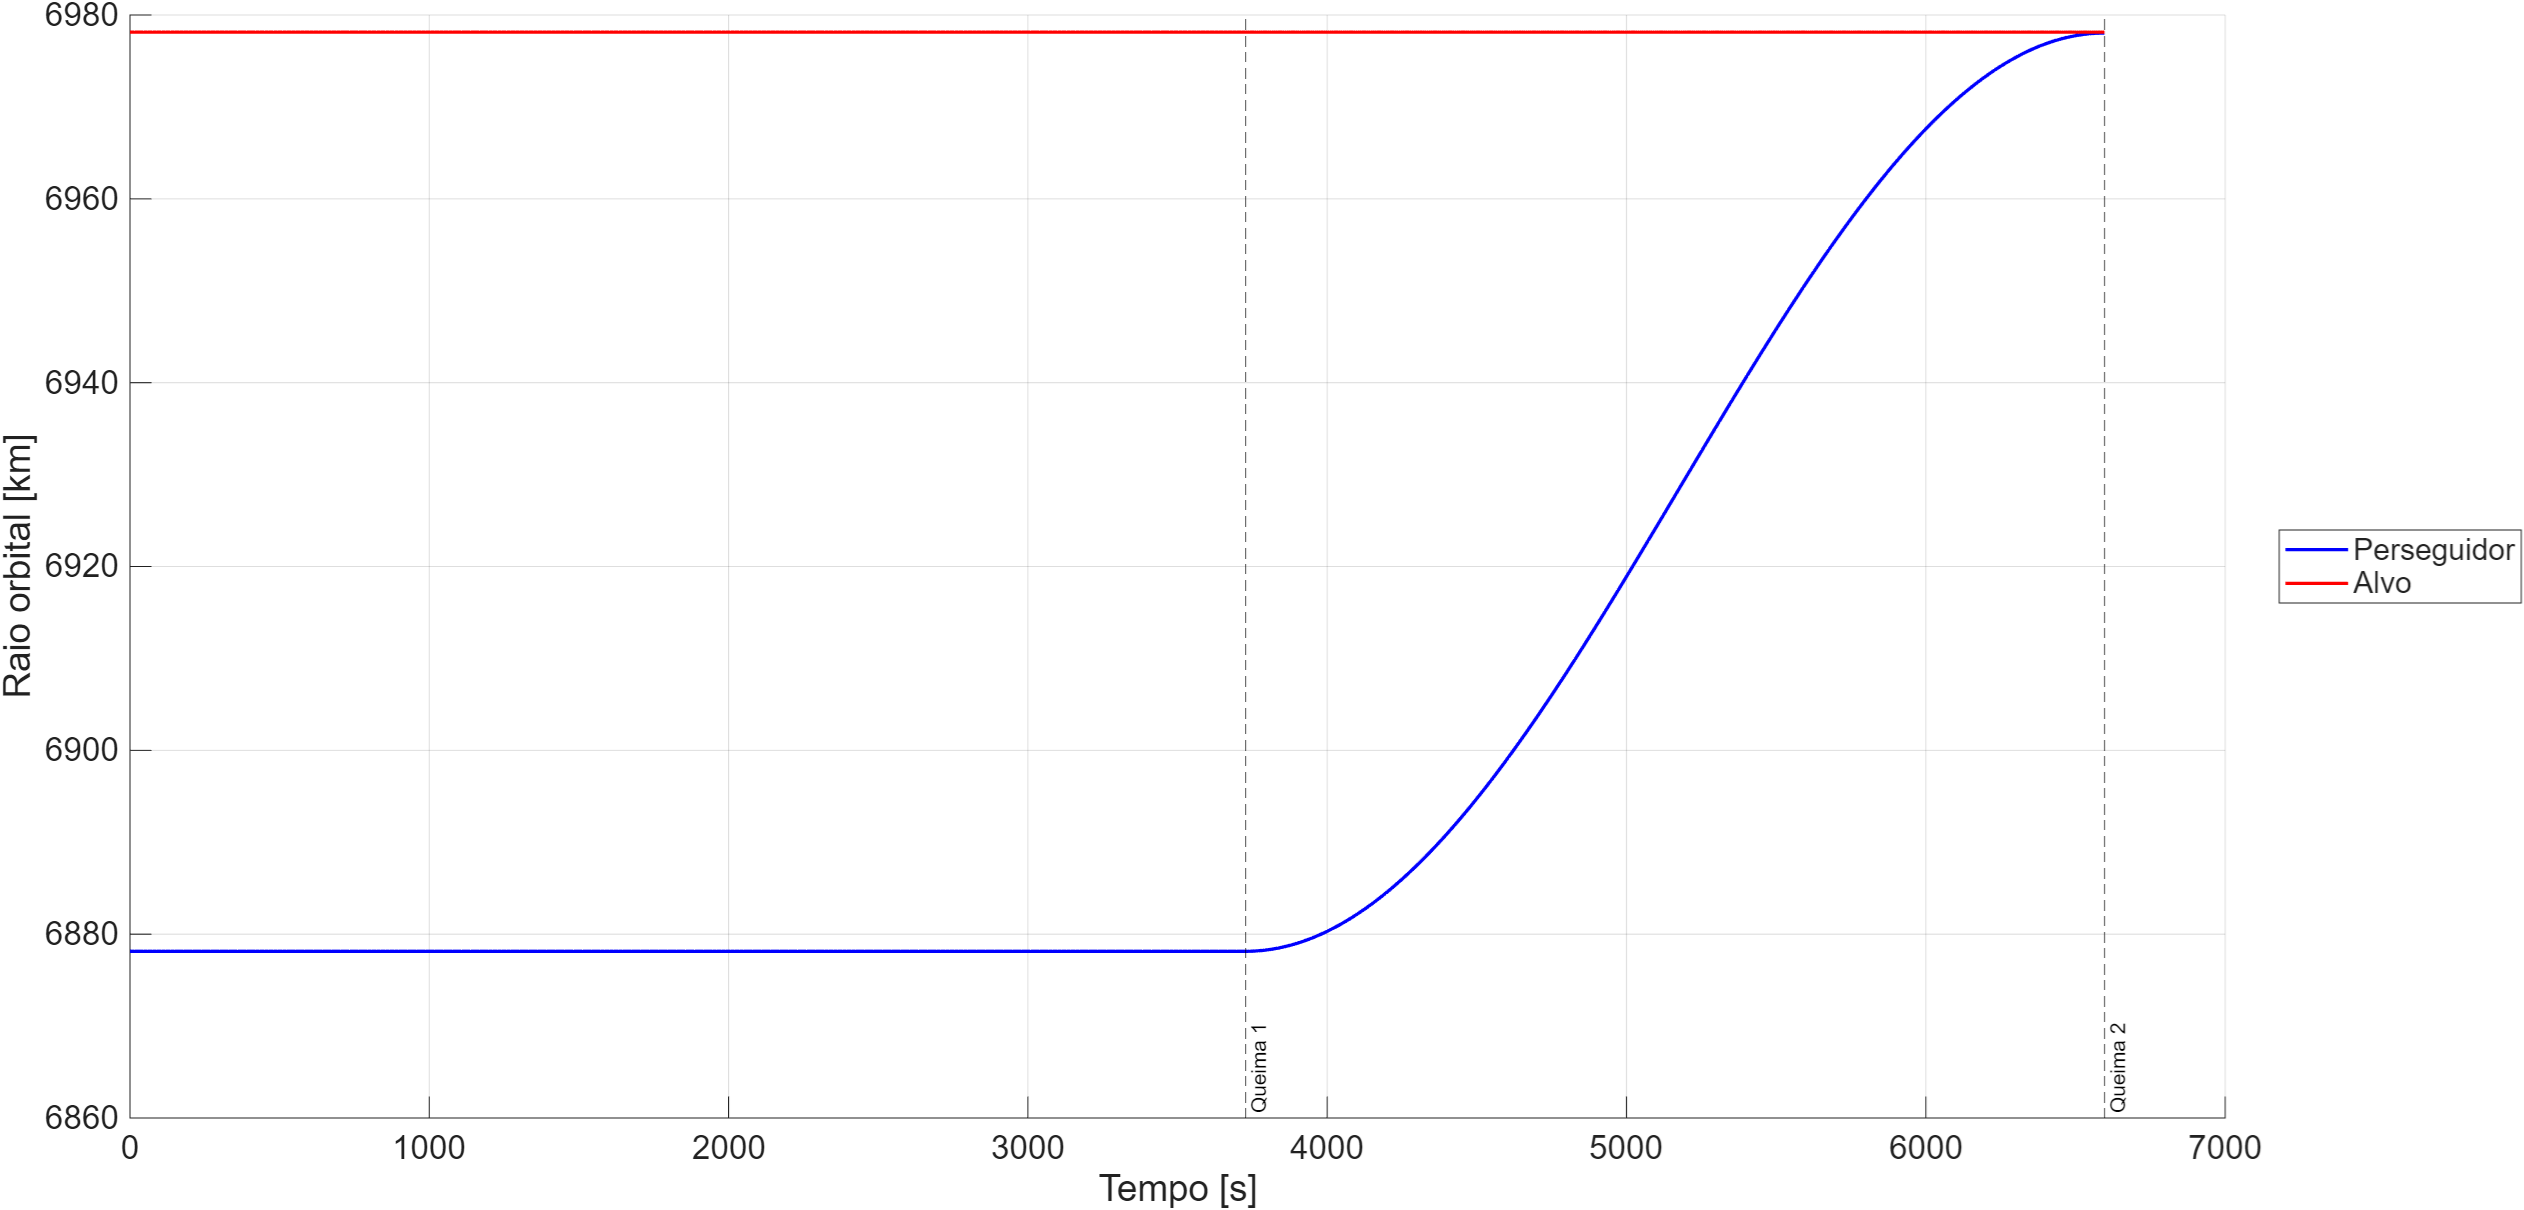
\includegraphics[width=1\linewidth]{4 Resultados e discussoes/Imagens/1 App longa distancia/3 Raio orbital ao longo do tempo.png}
\caption{Evolução do raio orbital do perseguidor ao longo do tempo absoluto.}
    \label{fig:cap4_3_raio_orbital}
\end{figure}

Após a transferência de órbita, o perseguidor está $100,0179$ metros abaixo do alvo (eixo radial), ou seja, nova altitude de $599,899$ km (raio orbital de $6.978,03$ km).

\subsection{Consumo de Delta-V}

A transferência de Hohmann requer dois impulsos. A Tabela~\ref{tab:cap4_deltav} apresenta, para cada queima, o instante de ocorrência e o correspondente consumo de $\Delta v$.

\begin{table}[H]
\centering
\caption{Consumo de Delta-V}
\begin{tabularx}{\linewidth}{|>{\centering\arraybackslash}X|>{\centering\arraybackslash}X|>{\centering\arraybackslash}X|}
\hline
\multicolumn{1}{|c|}{\textbf{Delta-V}} &
\multicolumn{1}{c|}{\textbf{[m/s]}} &
\multicolumn{1}{c|}{\textbf{Instante de tempo [s]}} \\
\hhline{|=|=|=|}
Consumo de $\Delta v_1$      & $27,39$ & $3.728$ \\
\hline
Consumo de $\Delta v_2$      & $27,29$ & $6.598$ \\
\hline
\textbf{Consumo de $\Delta v$ total}  & $54,69$ & -       \\
\hline
\end{tabularx}
\label{tab:cap4_deltav}
\end{table}

% \subsection{Distância relativa}

% A Figura~\ref{fig:cap4_4_dist_relativa} apresenta a evolução temporal da distância relativa. O \emph{drift} gerado pela diferença de velocidade orbital promove a aproximação gradual desde o início da aproximação de longa distância.

% \begin{figure}[H]
% \centering
% 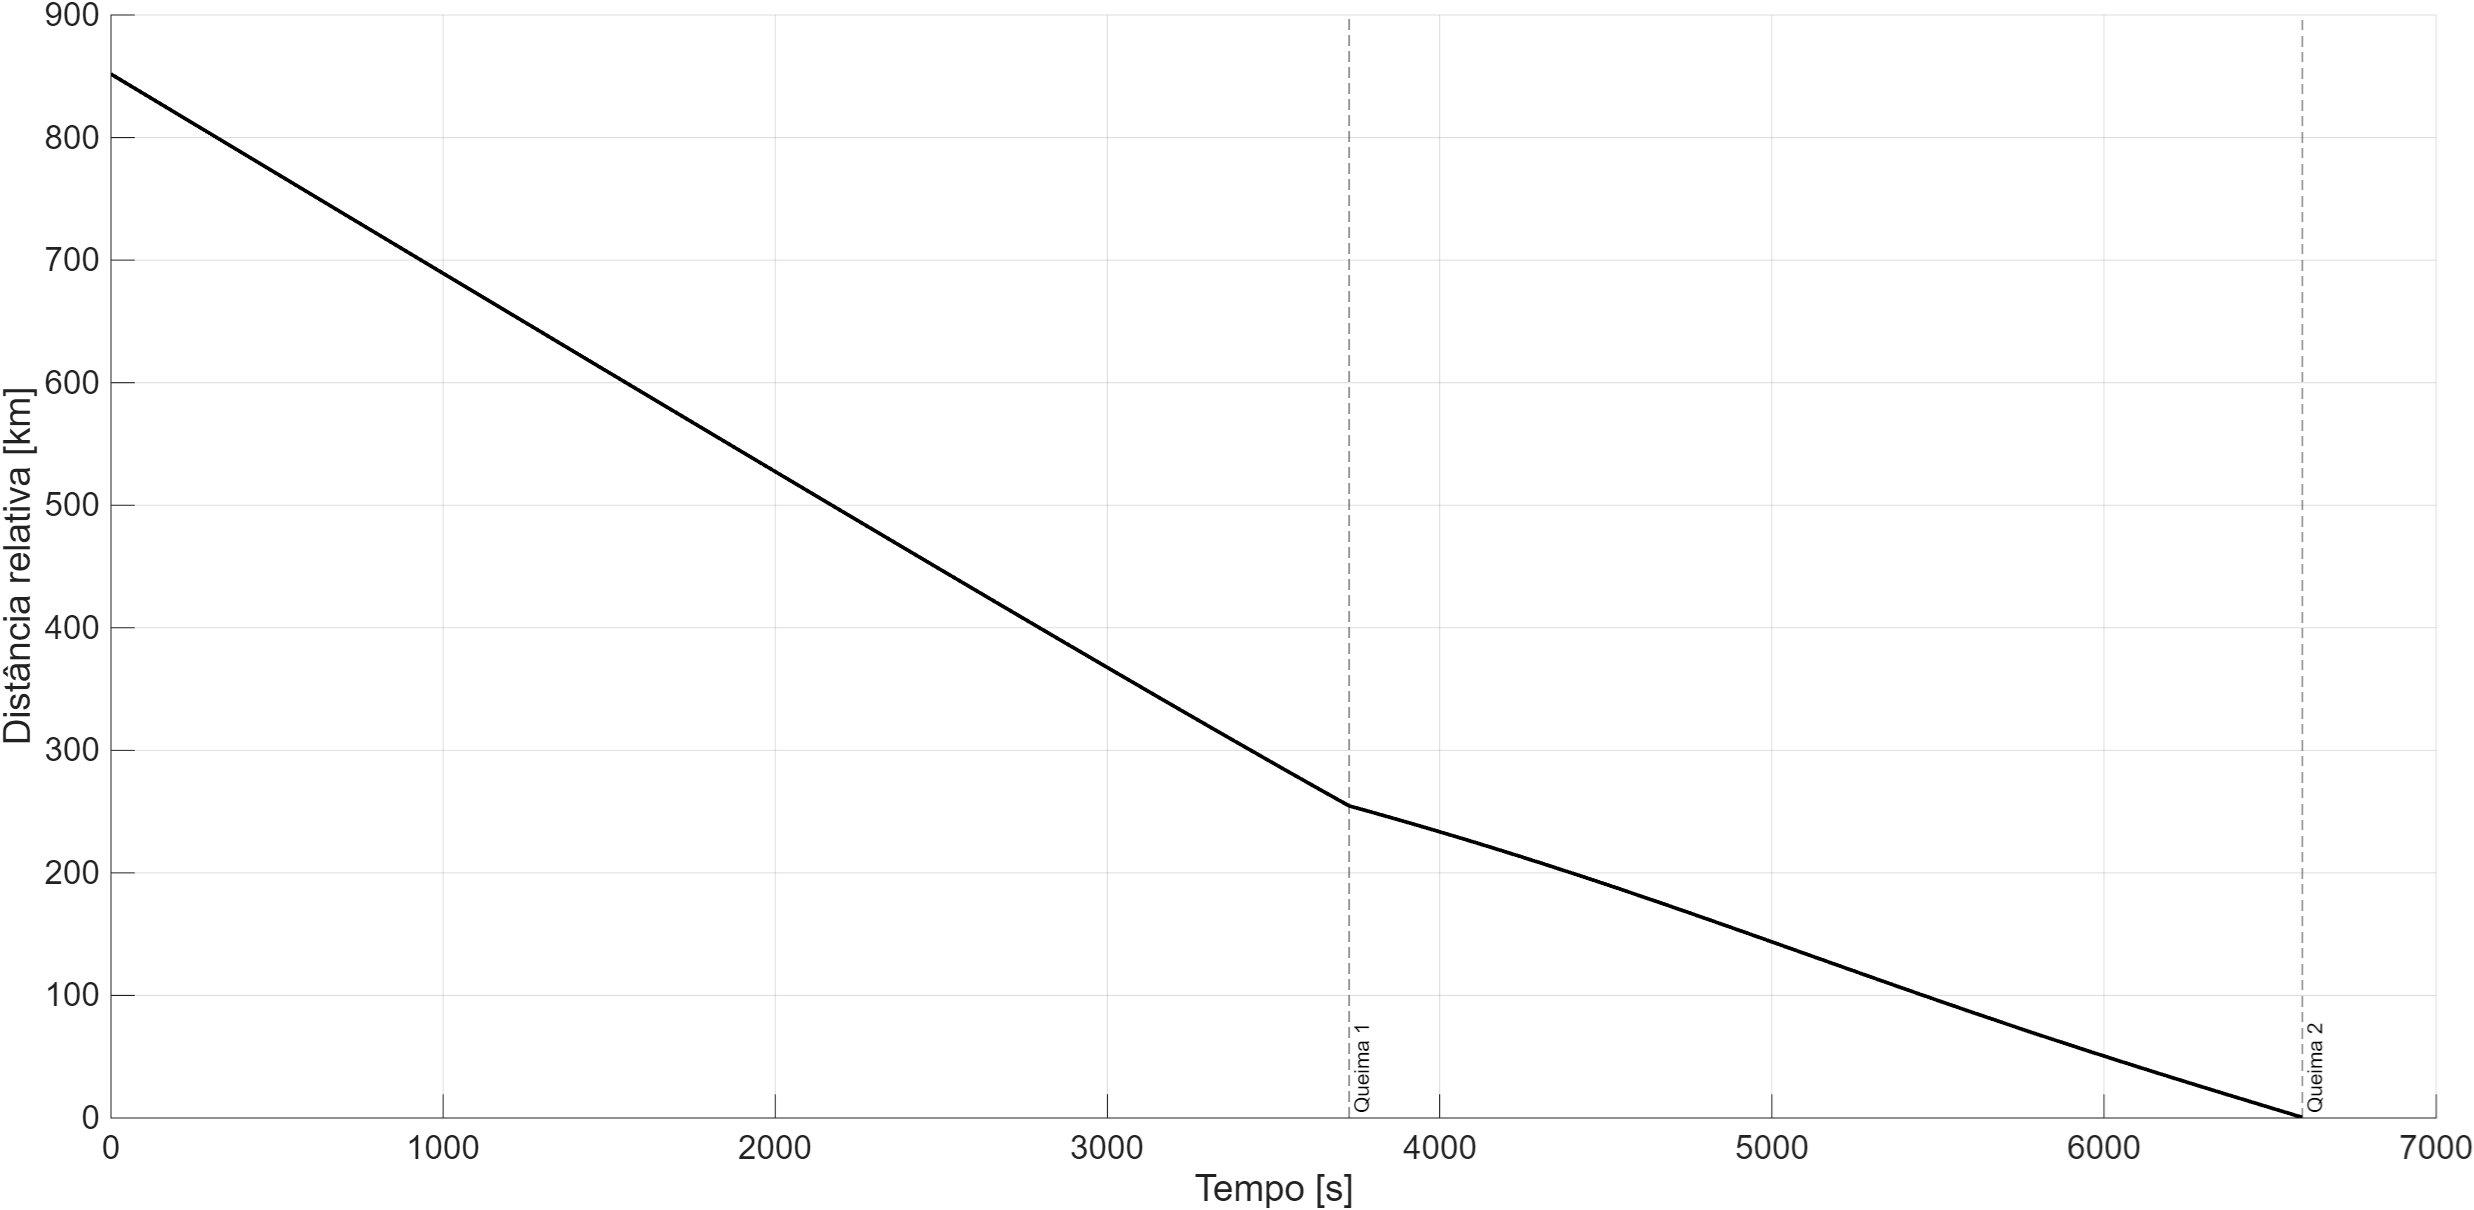
\includegraphics[width=1\linewidth]{4 Resultados e discussoes/Imagens/1 App longa distancia/4 Distância relativa ao longo do tempo.png}
% \caption{Evolução da distância relativa entre as espaçonaves no referencial ECI.}
%     \label{fig:cap4_4_dist_relativa}
% \end{figure}

% Para melhor visualização, a Tabela~\ref{tab:cap4_dist_relativa_eci} apresenta as distâncias relativas em determinados instantes de tempo, os mesmos utilizados anteriormente.

% \begin{table}[H]
% \centering
% \caption{Distância relativa em ECI nos instantes principais}
% \begin{tabularx}{\linewidth}{|>{\centering\arraybackslash}X|>{\centering\arraybackslash}X|>{\centering\arraybackslash}X|}
% \hline
% \multicolumn{1}{|c|}{\textbf{Instante de tempo [s]}} &
% \multicolumn{1}{c|}{\textbf{Distância relativa [km]}} &
% \multicolumn{1}{c|}{\textbf{Evento}} \\
% \hhline{|=|=|=|}
% $0$     & $851,774$ & Início da aproximação longa \\
% \hline
% $2.889$ & $385,079$ & — \\
% \hline
% $3.728$ & $254,678$ & Queima 1 \\
% \hline
% $6.598$ & $0,506$   & Queima 2 \\
% \hline
% \end{tabularx}
% \label{tab:cap4_dist_relativa_eci}
% \end{table}

\subsection{Cenários}

Para avaliar o desempenho da aproximação de longa distância, novas condições iniciais foram estabelecidas para obtenção de novas medidas.

\subsubsection{Condições iniciais}

Conforme a Tabela~\ref{tab:cap4_longitude_cenarios}, o primeiro cenário (A) possui as medidas e valores já apresentados até o momento, enquanto que o cenário (B) possui nova condição inicial para nova análise.

\begin{table}[H]
\centering
\caption{Longitude inicial do perseguidor por cenário}
\begin{tabularx}{\linewidth}{|>{\centering\arraybackslash}X|>{\centering\arraybackslash}X|}
\hline
\multicolumn{1}{|c|}{\textbf{Cenário}} &
\multicolumn{1}{c|}{\textbf{Longitude inicial do perseguidor}} \\
\hhline{|=|=|}
A & $-7^{\circ}$ ou $-0,1222$ (rad) \\
\hline
B & $-90^{\circ}$ [deg] ou $-1,5708$ (rad) \\
\hline
\end{tabularx}
\label{tab:cap4_longitude_cenarios}
\end{table}

A Figura~\ref{fig:cap4_posicoes_cenarios} exemplifica a posição do perseguidor em cada cenário.

\begin{figure}[H]
\centering
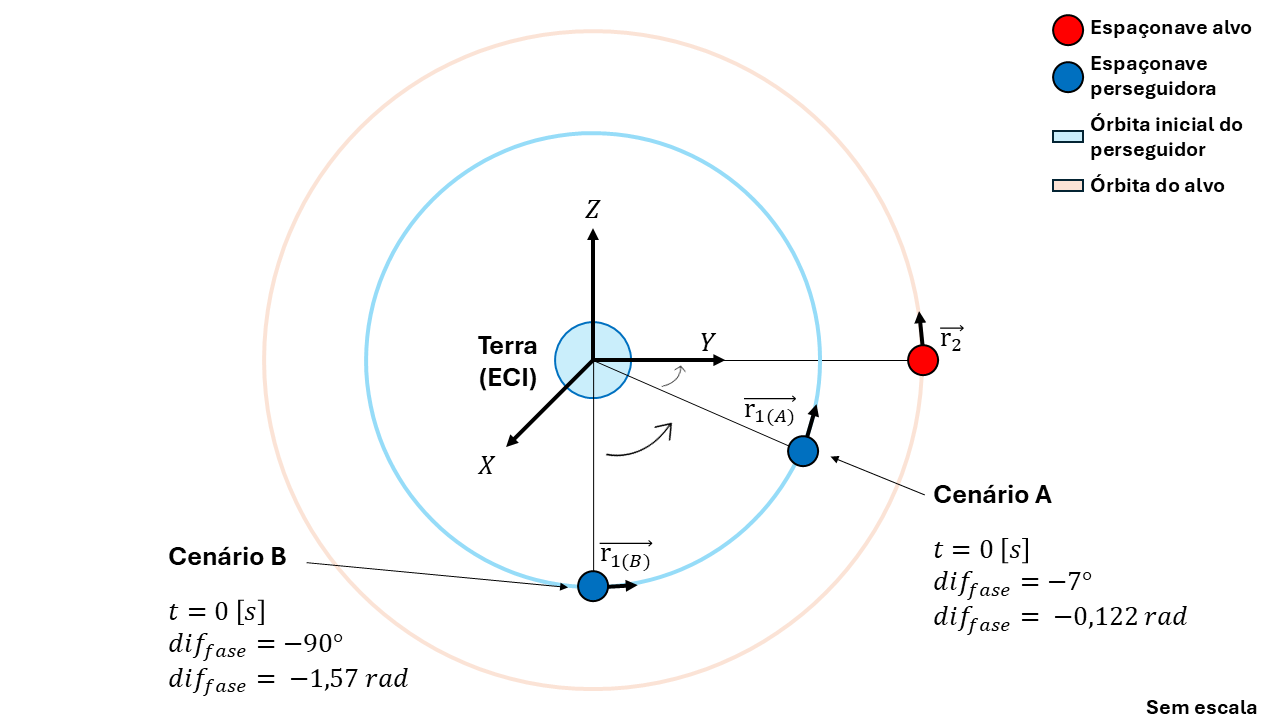
\includegraphics[width=1\linewidth]{3 Formulacao matematica/Imagens/Cenario A e B.png}
\caption{Posições iniciais do perseguidor em cada cenário.}
\label{fig:cap4_posicoes_cenarios}
\end{figure}

\subsubsection{Longitude no instante da queima}

Ao modificar a longitude inicial e o raio orbital inicial do perseguidor, os instantes de queima também foram alterados conforme apresentados nas Tabela~\ref{tab:cap4_longitudes_queimas} e Tabela~\ref{tab:cap4_longitudes_queimas_rad}.
Como as órbitas são keplerianas e o intervalo simulado é curto, não se espera influência consistente de perturbações; portanto, os valores não foram comparados entre si.

\begin{table}[H]
\centering
\caption{Longitudes na queima 1 e queima 2}
\begin{tabularx}{\linewidth}{|>{\raggedright\arraybackslash}X|
                             >{\raggedright\arraybackslash}c|
                             r|r|}
\hline
\multicolumn{1}{|c|}{\textbf{Variável}} &
\multicolumn{1}{c|}{\textbf{Unidade}} &
\multicolumn{1}{c|}{\textbf{Cenário A}} &
\multicolumn{1}{c|}{\textbf{Cenário B}} \\
\hhline{|=|=|=|=|}
Longitude do perseguidor na queima 1 & grau & 229,38 & 128,15 \\
\hline
Longitude do alvo na queima 1        & grau & 231,31 & 132,02 \\
\hline
Longitude do perseguidor na queima 2 & grau & 49,38  & 308,15 \\
\hline
Longitude do alvo na queima 2        & grau & 49,38  & 308,16 \\
\hline
\end{tabularx}
\label{tab:cap4_longitudes_queimas}
\end{table}

\begin{table}[H]
\centering
\caption{Longitudes na queima 1 e queima 2}
\begin{tabularx}{\linewidth}{|>{\raggedright\arraybackslash}X|
                             >{\raggedright\arraybackslash}c|
                             r|r|}
\hline
\multicolumn{1}{|c|}{\textbf{Variável}} &
\multicolumn{1}{c|}{\textbf{Unidade}} &
\multicolumn{1}{c|}{\textbf{Cenário A}} &
\multicolumn{1}{c|}{\textbf{Cenário B}} \\
\hhline{|=|=|=|=|}
Longitude do perseguidor na queima 1 & radiano & 4,0034   & 2,2367   \\
\hline
Longitude do alvo na queima 1        & radiano & 4,0372   & 2,3041   \\
\hline
Longitude do perseguidor na queima 2 & radiano & 0,861774 & 5,378311 \\
\hline
Longitude do alvo na queima 2        & radiano & 0,861846 & 5,378383 \\
\hline
\end{tabularx}
\label{tab:cap4_longitudes_queimas_rad}
\end{table}

\subsubsection{Comparativo entre os cenários}

A Tabela~\ref{tab:cap4_comp_alt_tempos} apresenta novos valores de altitude e tempos obtidos após a mudança nos parâmetros iniciais do perseguidor durante a fase de aproximação de longa distância.

\begin{table}[H]
\centering
\caption{Comparação de altitude e tempos entre cenários}
\begin{tabularx}{\linewidth}{|>{\raggedright\arraybackslash}X|
                             >{\raggedright\arraybackslash}c|
                             r|r|r|r|}
\hline
\multicolumn{1}{|c|}{\textbf{Variável}} &
\multicolumn{1}{c|}{\textbf{Unidade}} &
\multicolumn{1}{c|}{\textbf{Cenário A}} &
\multicolumn{1}{c|}{\textbf{Cenário B}} &
\multicolumn{1}{c|}{\textbf{Diferença}} &
\multicolumn{1}{c|}{\textbf{Diferença (\%)}} \\
\hhline{|=|=|=|=|=|=|}
Altitude inicial do perseguidor      & km     & 500,00 & 400,00 & -100,00 & -20\% \\
\hline
Altitude do perseguidor após TH      & km     & 599,90 & 599,90 & 0,00    & 0\%   \\
\hline
Altitude do alvo                     & km     & 600,00 & 600,00 & 0,00    & 0\%   \\
\hline
Tempo até a queima 1                 & segundo& 3.728  & 31.134 & 27.406  & 735\% \\
\hline
Tempo de transferência orbital       & segundo& 2.870  & 2.839  & -31     & -1\%  \\
\hline
Tempo até a queima 2                 & segundo& 6.597  & 33.972 & 27.375  & 415\% \\
\hline
Tempo de drift                       & segundo& 900    & 900    & 0       & 0\%   \\
\hline
Tempo total (após drift)             & segundo& 7.471  & 34.873 & 27.375  & 365\% \\
\hline
\end{tabularx}
\label{tab:cap4_comp_alt_tempos}
\end{table}

O tempo total da aproximação de longa distância (desde a injeção do perseguidor em sua órbita inicial até o instante final do \emph{drift} orbital) no cenário (A) foi de $7.471$~s, enquanto no cenário (B) foi de $34.873$~s.
Em termos relativos, isso representa um aumento de $366{,}8\%$ em relação ao cenário (A), obtido pela comparação direta dos tempos totais:

\begin{equation}
\frac{34.873 - 7.471}{7.471}\times 100 \approx 366{,}8\%.
\end{equation}

Essa diferença se dá, pois no cenário (B), a condição de fase a ser atingida antes do início da manobra de curta distância exige um intervalo maior de deriva (\emph{drift}) para acumular a separação angular desejada, dado que essa etapa depende da diferença de movimento médio entre as espaçonaves.

\subsubsection{Consumo de Delta-V}
Outro parâmetro analisado foi o consumo de $\Delta v$.
Os parâmetros obtidos estão na Tabela~\ref{tab:cap4_comp_deltav} e foram calculados através da equação \emph{vis-viva}, ver \ref{eq:vis_viva}.
Pode-se notar que no cenário (B) houve um consumo maior de $\Delta v$, ao todo, $102\%$ a mais que o cenário (A).

\begin{table}[H]
\centering
\caption{Comparação de consumo de delta v entre cenários}
\begin{tabularx}{\linewidth}{|>{\raggedright\arraybackslash}X|
                             >{\raggedright\arraybackslash}c|
                             r|r|r|r|}
\hline
\multicolumn{1}{|c|}{\textbf{Variável}} &
\multicolumn{1}{c|}{\textbf{Unidade}} &
\multicolumn{1}{c|}{\textbf{Cenário A}} &
\multicolumn{1}{c|}{\textbf{Cenário B}} &
\multicolumn{1}{c|}{\textbf{Diferença}} &
\multicolumn{1}{c|}{\textbf{Diferença (\%)}} \\
\hhline{|=|=|=|=|=|=|}
Consumo de $\Delta v1$        & m/s & 27,39 & 55,52  & 28,13 & 103\% \\
\hline
Consumo de $\Delta v2$        & m/s & 27,29 & 55,12  & 27,83 & 102\% \\
\hline
Consumo total de $\Delta v$   & m/s & 54,69 & 110,63 & 55,94 & 102\% \\
\hline
\end{tabularx}
\label{tab:cap4_comp_deltav}
\end{table}

\subsubsection{Elementos orbitais}

Os elementos orbitais, apresentados na Tabela~\ref{tab:cap4_elementos_perseguidor}, foram coletados no final da aproximação de longa distância e não foram alterados.
Portanto, isso não refletirá em uma mudança significativa das condições iniciais para o movimento relativo descrito pelas equações \gls{hcw} que serão abordadas mais a frente.


\begin{table}[H]
\centering
\caption{Elementos orbitais do perseguidor}
\begin{tabularx}{\linewidth}{|>{\raggedright\arraybackslash}X|
                             >{\raggedright\arraybackslash}c|
                             r|r|}
\hline
\multicolumn{1}{|c|}{\textbf{Elemento orbital do perseguidor}} &
\multicolumn{1}{c|}{\textbf{Unidade}} &
\multicolumn{1}{c|}{\textbf{Cenário A}} &
\multicolumn{1}{c|}{\textbf{Cenário B}} \\
\hhline{|=|=|=|=|}
Semi-eixo maior (a) & km   & 6.978,04 & 6.978,04 \\
\hline
Excentricidade (e)  &      & 0        & 0        \\
\hline
Inclinação (i)      & grau & 0        & 0        \\
\hline
Ascensão reta do nó ascendente ($\Omega$) & grau & 0 & 0 \\
\hline
Argumento do perigeu ($\omega$) & grau & 0 & 0 \\
\hline
Anomalia verdadeira ($\nu$) & grau & 0 & 0 \\
\hline
\end{tabularx}
\label{tab:cap4_elementos_perseguidor}
\end{table}

No Apêndice~\ref{ap:ApendiceA} são apresentadas as posições e velocidades no referencial inercial.
A seguir serão apresentados os resultados da aproximação de curta distância.